\section{QuickDough Framework}\label{sec:framework}

\subsection{System Context}
This work assumes a hybrid computing architecture with both general purpose processor and FPGA, where the processor handles complex control intensive tasks such as providing the OS environment and FPGA focuses on compute intensive kernels. \figref{fig:typical-FPGA-accelerator} shows a typical FPGA acceleration system used in this paper. FPGA is attached to the system interconnection and it includes a group of independent accelerators customized for different compute kernels of the target application. In each accelerator, there are input/output data buffers used for buffering the communication data, a computation core customized for the compute kernels and an Acc-Ctrl block which can be used to start the computation core and acknowledge the computation core status as well. 

\begin{figure}[H]
    \center{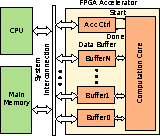
\includegraphics[width=0.85\linewidth]{typical-FPGA-accelerator}}
    \caption{Typical FPGA Acceleration System and Accelerator Architecture}
    \label{fig:typical-FPGA-accelerator}
\end{figure}

\subsection{QuickDough}
On top of the system context, QuickDough, an SCGRA based FPGA accelerator design methodology, is presented in \figref{fig:framework}. It starts from HW/SW partition where the compute intensive kernels of an application are identfied. Then it transforms the compute kernels in high level language program to DFGs for SCGRA compilation. There are already intensive work on both the HW/SW partition and DFG generation \cite{Baleani2002HW-SW} \cite{ROCCC}. We may automate the two steps in future, but currently we just manually handle the two steps in our preliminary research stage. 

After the HW/SW partition and DFG generation, the design methodology in \figref{fig:framework} can roughly be split  into two parts. The part on the top half is mainly responsible for the conventional software compilation targeting general purpose processor of the hybrid compute system. In order to make use of the FPGA accelerators, we need to replace the original compute kernels with the accelerator drivers before the standard software compilation. When the software compilation is completed, the binary code targeting the processor will be generated. 

The part on the bottom half mainly focuses on the SCGRA customization and compilation. Once the DFGs to be implemented on the SCGRA overlay are determined, SCGRA configuration such as operation type, PE pipeline, SCGRA size, on chip buffer capacity etc. should be decided accordingly. As the design space is large, delicate optimization algorithm is required to tackle the customization problem. At the moment, we just support the operation type customization and leave the rest design customization for future work. After the SCGRA customization, the SCGRA configuration can be decided and corresponding SCGRA compilation starts. If the SCGRA configuration is not available in the SCGRA library, hardware implementation is performed. After the implementation, the pre-implemented SCGRA will be put into the SCGRA library for reuse. Meanwhile, with the input DFG, SCGRA configuration and implementation, FPGA bitstream can be produced. When both the binary code and bitstream are ready, we complete the application specific FPGA acceleration system. 

\begin{figure}[H]
    \center{\includegraphics[width=0.9\linewidth]{framework}}
    \caption{QuickDough: FPGA Accelerator Design Methodology Using SCGRA Overlay}
    \label{fig:framework}
\end{figure}

